\subsection{Restore en un Cliente Linux}

Para ilustrar el proceso de restauración, he creado cinco archivos de texto y he calculado el \texttt{md5sum} de dos de ellos que luego serán eliminados y restaurados.

\begin{figure}[H]
    \centering
    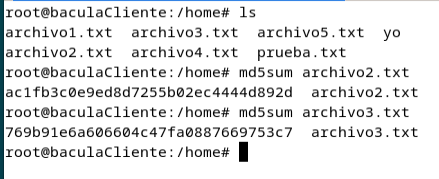
\includegraphics[width=0.5\linewidth]{instalacionBacula/5ARCHIVOS.png}
    \caption{Creacion de archivos y checksum.}
\end{figure}

Primero, realizamos el respaldo de los archivos en el sistema Bacula:
\begin{figure}[H]
    \centering
    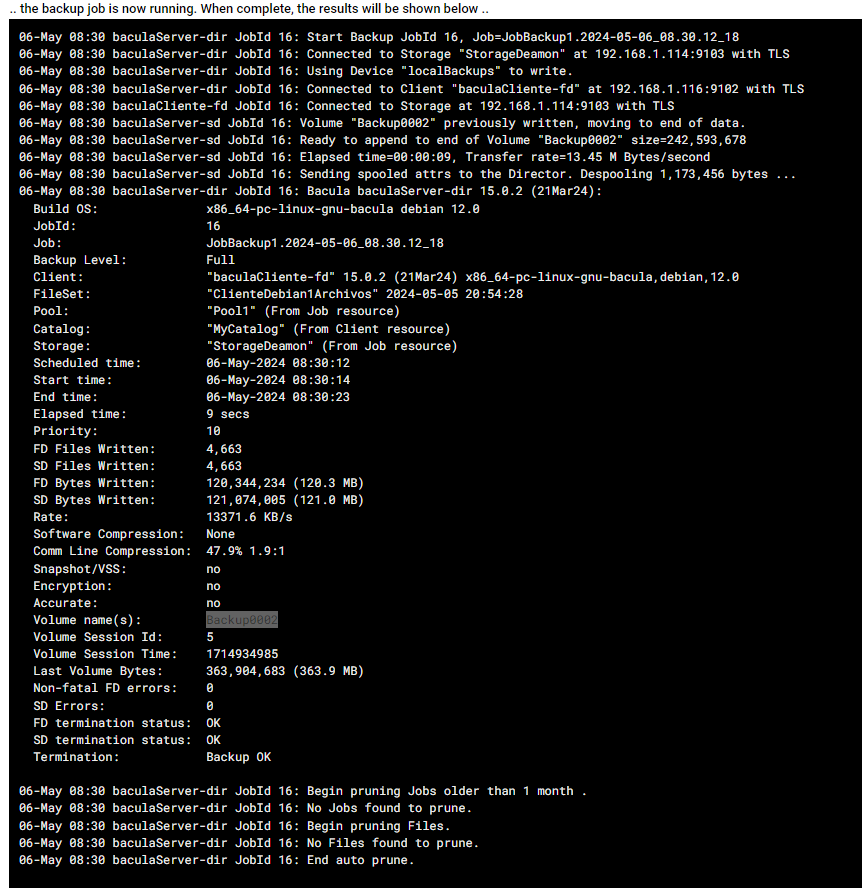
\includegraphics[width=0.5\linewidth]{instalacionBacula/backup0002.png}
    \caption{Realizando el respaldo de los archivos en Bacula.}
\end{figure}

Luego, eliminamos los archivos \texttt{archivo2.txt} y \texttt{archivo3.txt}:
\begin{figure}[H]
    \centering
    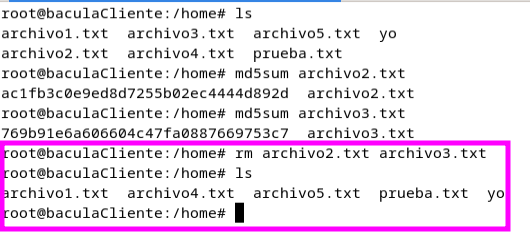
\includegraphics[width=0.5\linewidth]{instalacionBacula/rmArchivo23.png}
    \caption{Eliminación de los archivos que serán restaurados.}
\end{figure}

Procedemos con la restauración de los archivos eliminados:
\begin{figure}[H]
    \centering
    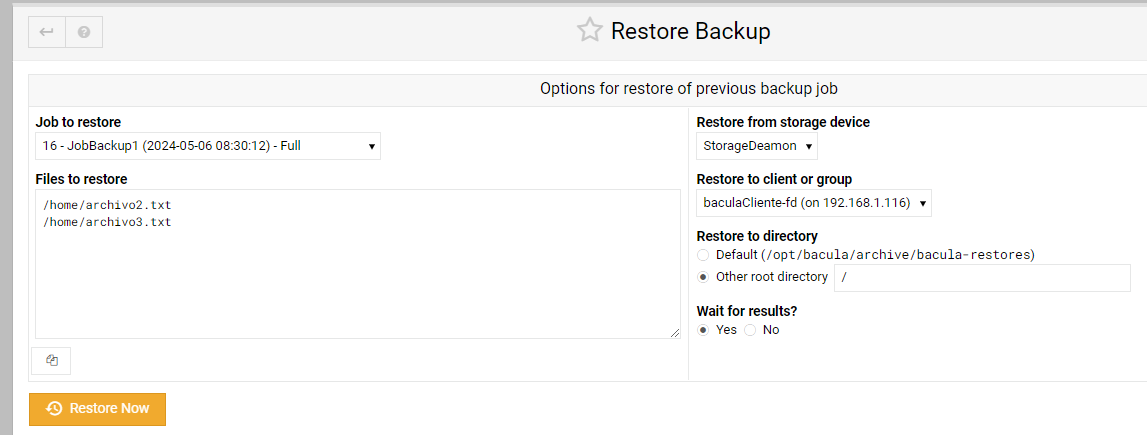
\includegraphics[width=0.5\linewidth]{instalacionBacula/resBackup.png}
    \caption{Configuración del proceso de restauración en Bacula.}
\end{figure}

Opciones para la restauración:
\begin{itemize}
    \item \textbf{Files to restore}: \texttt{/home/archivo2.txt}, \texttt{/home/archivo3.txt}
    \item \textbf{Restore from storage device}: \texttt{StorageDeamon}
    \item \textbf{Restore to client or group}: \texttt{baculaCliente-fd} (en 192.168.1.116)
    \item \textbf{Restore to directory}: opción por defecto (\texttt{/opt/bacula/archive/bacula-restores}) o directorio raíz (\texttt{/})
    \item \textbf{Wait for results}: Sí
\end{itemize}

\begin{figure}[H]
    \centering
    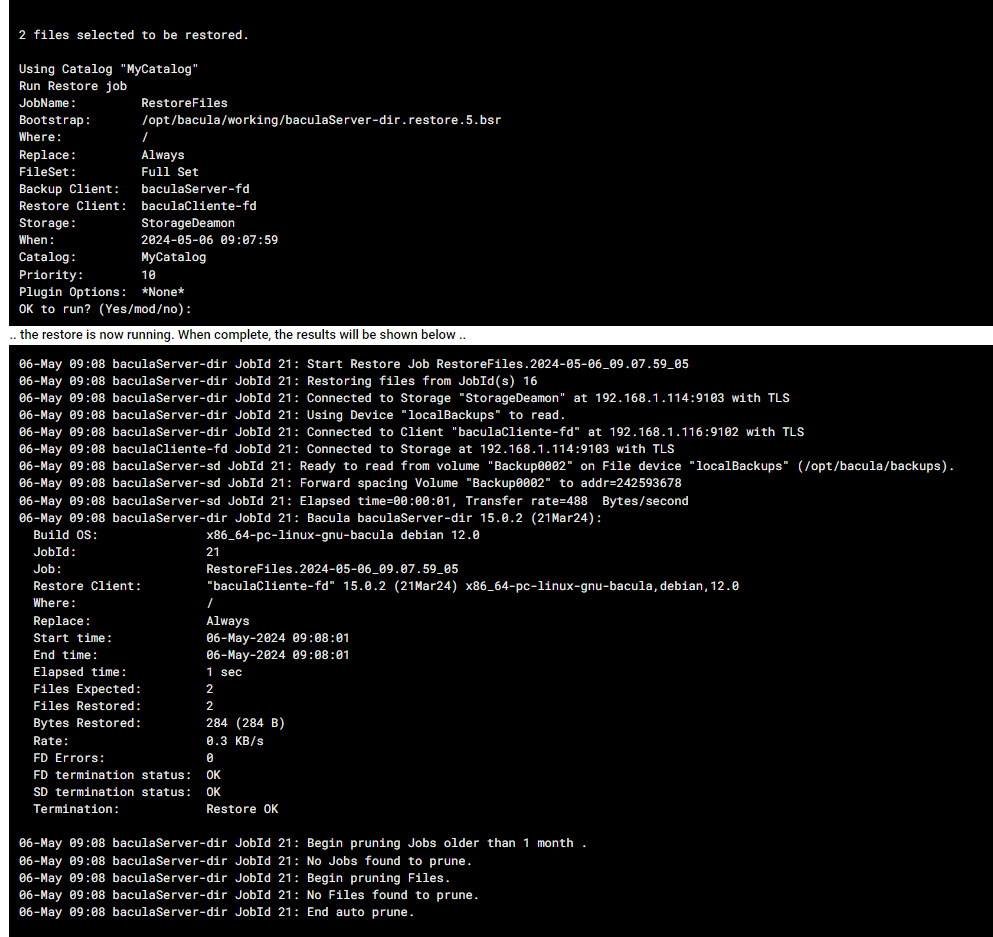
\includegraphics[width=0.5\linewidth]{instalacionBacula/restoresalidawebmin.png}
    \caption{salida de la restauración.}
\end{figure}

Una vez completada la restauración, confirmamos que los archivos han sido correctamente restaurados y verificamos su integridad:
\begin{figure}[H]
    \centering
    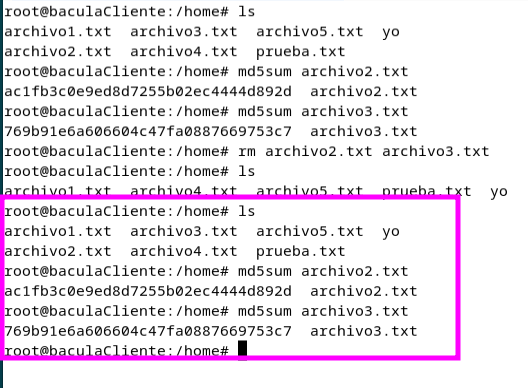
\includegraphics[width=0.5\linewidth]{instalacionBacula/restoreSusc.png}
    \caption{Verificación de los archivos restaurados en el cliente Linux.}
\end{figure}
